% !TeX program = xelatex
\documentclass[9pt]{beamer}
\usepackage{xcolor}
\definecolor{orange}{HTML}{80B395}
\definecolor{green}{HTML}{A5CC6B}
\definecolor{red}{HTML}{AC454A}
\definecolor{brown}{HTML}{EAD296}
\definecolor{darkgrey}{HTML}{313630}
\definecolor{lightgray}{HTML}{AAAAAA}
\definecolor{cornflower}{HTML}{247BA0}
\definecolor{sienna}{HTML}{6C464F}
\usefonttheme{professionalfonts} % using non standard fonts for beamer
\usefonttheme{serif} % default family is serif
\usepackage{fontspec}
\usepackage{setspace}
\usepackage{natbib}
\usepackage{animate}
\usepackage{tikz}
\usepackage{graphicx}
%\usepackage[T1]{fontenc}

\bibliographystyle{abbrv}
%\setmainfont{Liberation Serif}
%\setmainfont{Liberation Serif}
\setmainfont{Comfortaa}
%\usepackage[T1]{fontenc}

\setbeamercolor{frametitle}{bg=orange,fg=white}
\setbeamercolor{author in head/foot}{bg=orange,fg=white}

%\setbeamerfont{page number}{size=\Huge}

%\setbeamertemplate{itemize itemjpegs}[circle]
\useinnertheme{circles}
\setbeamercolor{palette primary}{bg=orange,fg=white}
%\setbeamercolor{palette secondary}{bg=red,fg=white}
\setbeamertemplate{itemize item}{\color{darkgrey}$\circ$}
\setbeamercolor{structure}{fg=darkgrey} % itemize, enumerate, etc

%\setbeamercolor{section in head/foot}{bg=red}
\setbeamercolor{title}{fg=orange} %, bg=brown
\setbeamercolor{author}{fg=darkgrey}
\setbeamercolor{institute}{fg=darkgrey}
\setbeamercolor{date}{fg=darkgrey}
%\setbeamercolor{normal text}{fg=darkgrey}
\makeatletter
\setbeamertemplate{headline}{%
	\usebeamercolor[bg]{frametitle}\rule{\textwidth}{1cm}
}
\setbeamerfont{title}{size=\LARGE}
\setbeamerfont{institute}{size=\normalsize}
\renewcommand*{\bibfont}{\scriptsize}


\setbeamertemplate{frametitle}{%
	\vskip-1cm%
	\begin{minipage}[c][\headheight][c]{\textwidth}%
		\usebeamerfont{frametitle}
		\strut\insertframetitle\par
		{%
			\ifx\insertframesubtitle\@empty%
			\else%
			{\usebeamerfont{framesubtitle}\usebeamercolor[fg]{framesubtitle}\strut\insertframesubtitle\par}%
			\fi
		}%      
		\vspace*{0.05cm}
	\end{minipage}%
	\vskip-0.1em
}
%\setbeamertemplate{footline}{%
%	\leavevmode%
%	\hbox{\begin{beamercolorbox}[wd=\paperwidth,ht=4.5ex,dp=3.125ex]{author in head/foot}%
%			\usebeamerfont{author in head/foot} bar
%	\end{beamercolorbox}}%
%	\vskip0pt%
%}
\makeatother


\title{Loss Landscape \\ Visualization}
\author{Talk by Stefan Wezel}
\institute{Optimization and Neural Architecture Search}

\date{\today}


%\setbeamertemplate{sidebar right}{}
%\setbeamertemplate{footline}{%
%	\hfill\usebeamertemplate***{navigation symbols}
%	\hspace{1cm}\insertframenumber{}}
\setbeamerfont{page number in head/foot}{size=\small}
    \setbeamertemplate{footline}{%
	\raisebox{5pt}{\makebox[\paperwidth]{\hfill\makebox[10pt]{\scriptsize\insertframenumber}}}}
\setbeamertemplate{navigation symbols}{}
%\onehalfspacing
\setstretch{1.3}
\begin{document}
	

\setbeamercolor{background canvas}{bg=white}
\setbeamercolor{normal text}{fg=darkgrey}
\usebeamercolor[fg]{normal text}
\begin{frame}[plain]
	\titlepage
\end{frame} 



\setbeamercolor{background canvas}{bg=white}
\setbeamercolor{normal text}{fg=darkgrey}
\usebeamercolor[fg]{normal text}
\setbeamertemplate{itemize item}{\color{darkgrey}$\circ$}
\begin{frame}
\frametitle{Overview}
%\framesubtitle{}
\begin{itemize}%\setlength\itemsep{1.5em}
	\item Introduction
	\item Motivation
	\item Tools to inspect the loss landscape
	\item How does the landscape look like?
	\item How can we use those Findings?
	\begin{itemize}
		\item Two Examples
	\end{itemize}
	\item Summary and Discussion
\end{itemize}
\end{frame} 


\begin{frame}
\frametitle{Introduction}
%\framesubtitle{}
\begin{itemize}%\setlength\itemsep{1.5em}
	\item Deep neural nets (DNNs) have large parameter set $\theta$%are powerful, overparametrized function approximators
	\item We want to find optimal set of parameters $\theta^*$
	\item By minimizing $\mathcal{L}(X,Y;\theta)$
%	\item They are trained by optimizing their parameters $\theta$ according to some objective $\mathcal{L}(X,Y;\theta)$
%	\item Non-linearities prohibit closed form solution to find optimal set of parameters $\theta^*$
	\item No closed form solution
%	\item When I first heard about these things, I thought, well why don't we just set to zero and find optimum analytically, like in high school math?
%	\item Turns out... it is a bit harder than that
	\item We rely on iterative approaches
	\begin{itemize}
		\item Stochastic Gradient Descent (SGD), ADAM, ...
	\end{itemize}
%	\item Like were in the mountains and we are surrounded by fog
%	\item It would be much easier, if we could see the landscape around us
%	\item Due to this lack of knowledge how the loss function looks like, we need to rely on some iterative, algorithmic approach to find (local) optimum
%	\item Often SGD, ADAM, ...
	%\item Other approaches and challenges
	\begin{figure}
		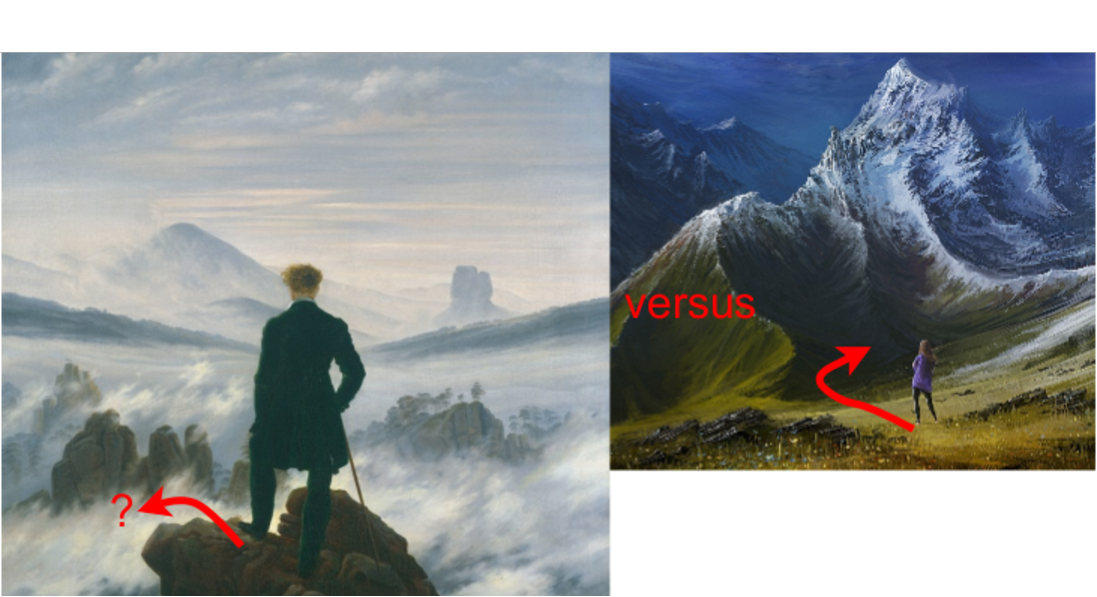
\includegraphics[width=.8\linewidth]{figures/llv.pdf}
	\end{figure}
\end{itemize}
\end{frame} 



\begin{frame}
\frametitle{Motivation}
%\framesubtitle{}
\begin{itemize}%\setlength\itemsep{1.5em}
	\item When designing a model
	\begin{itemize}
		\item What architecture, learning rate, ...
	\end{itemize}
%	\begin{itemize}
%		\item What architectures work well and why?
%		\item What learning rate?
%		\item What batch size?
%		\item What optimizer?
%		\item ... %no grid search
%	\end{itemize}
	\item Often rely on experience or anecdotal knowledge
	\item Loss landscape visualization could help build intuition and empirical knowledge
	\begin{itemize}
		\item What is the role of architecture?
		\item What is the effect of hyperparameters?
			\item Help understand generalization in DNNs
			\begin{itemize}
						\item Do flat minima really generalize better?
			\end{itemize}
	\end{itemize}
%	\item If there was some way to find empirical knowledge about this, it might help a lot
%	\item If there was some way to visualize what this loss function looks like, we could built better intuition about what works well
%	\item and not rely so much on anecdotal knowledge
%	\item -> Allows qualitative assessment of hyperparamters/training methods/architectures
%	\item -> Allows to find empirical results
%	\item So how ca
\end{itemize}
\end{frame} 

\begin{frame}
\frametitle{Methods}
\framesubtitle{Loss Landscape Visualization - But How?}
%\begin{center}
	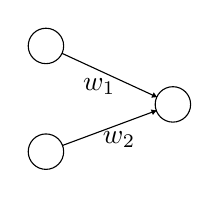
\begin{tikzpicture}[scale=0.075]
	\tikzstyle{every node}+=[inner sep=0pt]
	\draw [black] (18,-22.7) circle (3);
	\draw [black] (18,-40.6) circle (3);
	\draw [black] (39.5,-32.6) circle (3);
	\draw [black] (20.72,-23.95) -- (36.78,-31.35);
	\fill [black] (36.78,-31.35) -- (36.26,-30.56) -- (35.84,-31.46);
	\draw (27.02,-28.16) node [below] {$w_1$};
	\draw [black] (20.81,-39.55) -- (36.69,-33.65);
	\fill [black] (36.69,-33.65) -- (35.76,-33.46) -- (36.11,-34.39);
	\draw (30.39,-37.14) node [below] {$w_2$};
	\end{tikzpicture}
\begin{figure}
	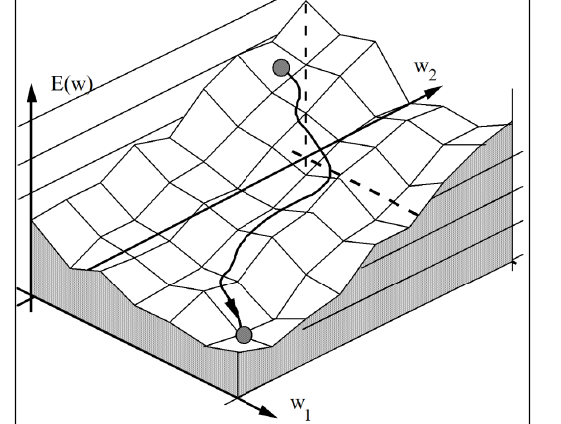
\includegraphics[width=.65\linewidth]{figures/two_weight_loss.png}
\end{figure}
\tiny\color{lightgray}Image source: Introduction to Neural Networks - A. Zell
\end{frame}


\begin{frame}
\frametitle{Methods}
\framesubtitle{Linear Interpolation - Idea}
\begin{itemize}%\setlength\itemsep{1.5em}
	\item Obvious problem: weight space is very high dimensional
	\item We need to find some visualizable subspace
	\item Goodfellow et al. propose:
	\begin{itemize}
		\item Linearly interpolate between two parameter sets $\theta_0$ and $\theta_1$
	\end{itemize}
	%\item Idea: at random location, sweep line(s)
	%\item -> span linear subspace
%	\item i.e. interpolate between them %trained and untrained
	\item Iteratively increase weight on $\theta_1$ (and reduce on $\theta_0$)
	\begin{itemize}
		\item Plot $f(\alpha) = \mathcal{L}((1-\alpha)\theta_0 + \alpha \theta_1)$
	\end{itemize}
\end{itemize}
\end{frame}

\begin{frame}
\frametitle{Methods}
\framesubtitle{Linear Interpolation - Results}
\begin{figure}
	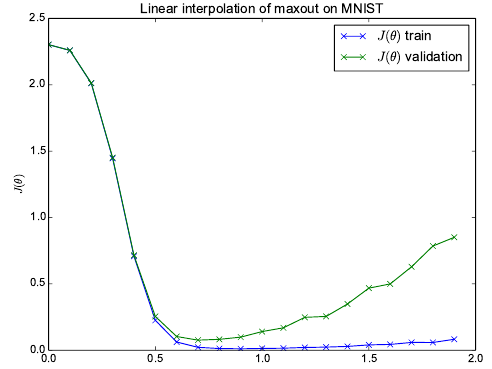
\includegraphics[width=.7\linewidth]{figures/linear_interpol_1.png}
%	\caption{}
\end{figure}
\begin{itemize}
	\item Interplolation between $\theta_{untrained}$ (left) and $\theta_{trained}$ (right)
	\item Loss is smooth (in this subspace)
%	\item Lot of time is spent exploring the
\end{itemize}
\tiny\color{lightgray}Image source: Qualitatively characterizing neural network optimization problems - Goodfellow et al.
\end{frame} 



\begin{frame}
\frametitle{Methods}
\framesubtitle{Linear Interpolation - Results}
\begin{itemize}
	\item Investigate other things
	\item I.e. the effect of batch size
	\item $\rightarrow$ increase weight on large batch size model
	\begin{figure}
		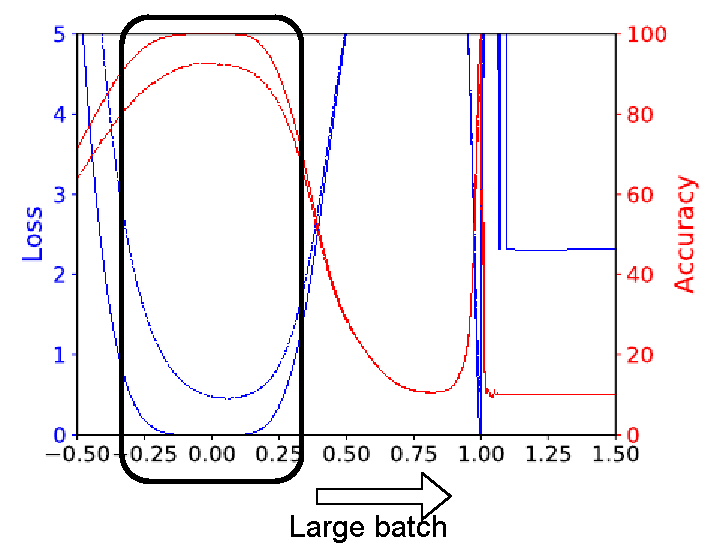
\includegraphics[width=0.7\linewidth]{figures/batch_size_1.pdf}
		%\caption{$\rightarrow$ increase weight on large batch size model}
	\end{figure}
\item Model with smaller batch size has flatter minimum
\end{itemize}
\tiny\color{lightgray}Image source: Visualizing the loss landscape of neural nets - Li et al.
\end{frame} 
\begin{frame}
\frametitle{Methods}
\framesubtitle{Linear Interpolation - Results}
\begin{itemize}
	\item Investigate other things
	\item I.e. the effect of batch size
	\item $\rightarrow$ increase weight on large batch size model
	\begin{figure}
		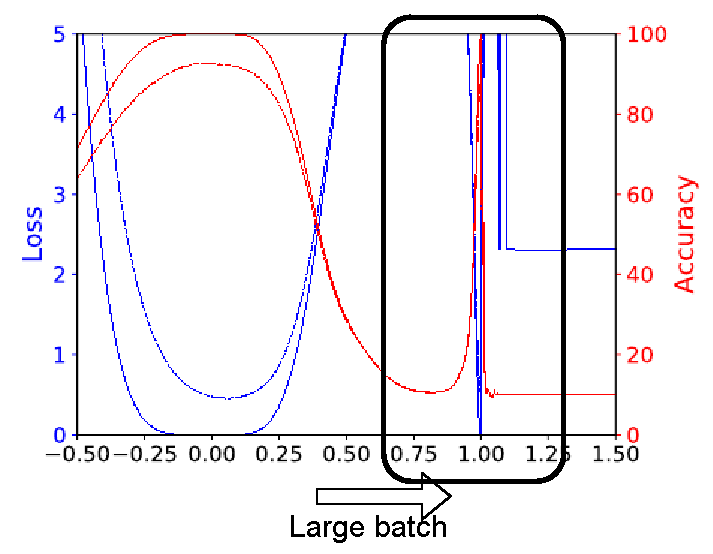
\includegraphics[width=0.7\linewidth]{figures/batch_size_2.pdf}
		%\caption{$\rightarrow$ increase weight on large batch size model}
	\end{figure}
	\item Model with smaller batch size has flatter minimum
\end{itemize}
\tiny\color{lightgray}Image source: Visualizing the loss landscape of neural nets - Li et al.
\end{frame}

\begin{frame}
\frametitle{Methods}
\framesubtitle{Linear Interpolation - Limitations}
\begin{itemize}
	\item 1-D interpolation subspace is limited
	\begin{itemize}
		\item Can it capture non-convexities?
	\end{itemize}
%	\item 1-D cannot really capture non-convexity (no local minima along the linear path)
	\item Does not consider norms of weights/filters
%	\item Does not consider batch normalization
	\item Can be misleading
\end{itemize}
\end{frame} 



\begin{frame}
\frametitle{Methods}
\framesubtitle{2D approaches - Random Directions}
\begin{itemize}%\setlength\itemsep{1.5em}
	\item Idea: Choose center point $\hat{\theta}$ and two direction vectors
	\begin{itemize}
	\item $f(\alpha, \beta) = \mathcal{L}(\hat{\theta }+ \alpha u_1 + \beta u_2)$
	\item plot loss at center + samples along directions
	\end{itemize}
	\item More expressive plots
	\item Problem: scaling behavior
	\item Scale of updates does not correspond to scale of weights
	\begin{itemize}
		\item Changes in weights can have too much/ too little effect
	\end{itemize}
	\item Distorted loss landscape
	\item Proposed solution by Li et al.:
	\begin{itemize}
		\item Filter normalization
	\end{itemize}
\end{itemize}
\end{frame} 

\begin{frame}
\frametitle{Methods}
\framesubtitle{2D approaches - Filter Normalization}
\begin{itemize}
	\item Pick random direction vectors $u_i$ 
	\item Normalize direction: $u_i \leftarrow \frac{||w||}{||u_i||}$
	\item Updates live on same scale as the weights
	\item Plot $f$ around centerpoint $\hat{\theta}$
	\item Compare different architectures, hyperparameters, ...
\end{itemize}
\end{frame}

\begin{frame}
\frametitle{Methods}
\framesubtitle{2D with Filter Normalization - Results}
\begin{figure}
	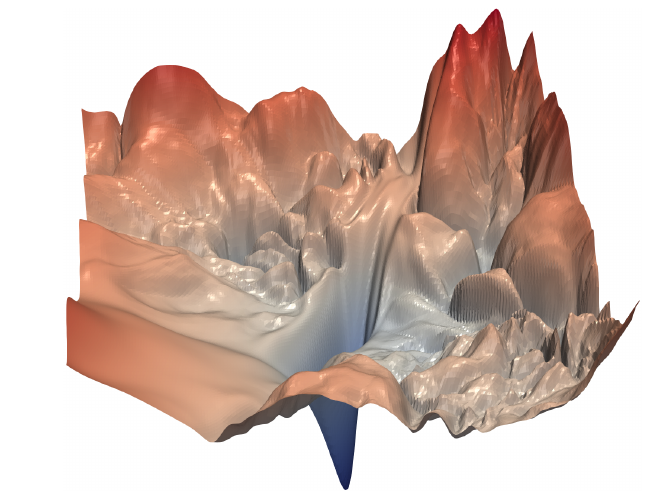
\includegraphics[width=0.8\linewidth]{figures/vgg_loss.png}
%	\caption{Without Skip connections}
\end{figure}
\begin{itemize}
	\item Convolutional neural net without skip connections
\end{itemize}
\tiny\color{lightgray}Image source: Visualizing the loss landscape of neural nets - Li et al.
\end{frame} 
\begin{frame}
\frametitle{Methods}
\framesubtitle{2D with Filter Normalization - Results}
\begin{figure}
	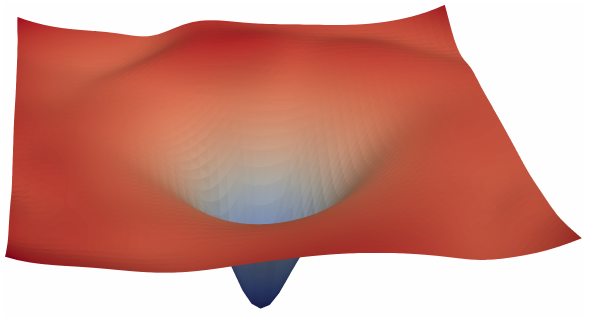
\includegraphics[width=\linewidth]{figures/resnet_loss.png}
%	\caption{With skip connections}
\end{figure}
\begin{itemize}
	\item Convolutional neural net with skip connections
\end{itemize}
\tiny\color{lightgray}Image source: Visualizing the loss landscape of neural nets - Li et al.
\end{frame}

\begin{frame}
\frametitle{Methods}
\framesubtitle{2D with Filter Normalization - Results}
\begin{figure}
	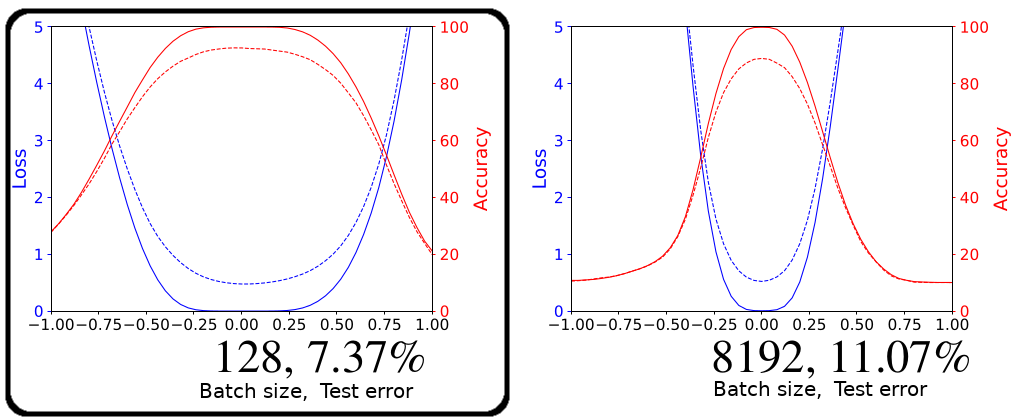
\includegraphics[width=.85\linewidth]{figures/batch_size_normalized_1.png}
	%\caption{Loss landscape around $\hat{\theta }$ for two models trained on different batch sizes.}
\end{figure}
\begin{itemize}
	\item Loss landscape around $\hat{\theta }$
	\item For batch size $128$ versus $8192$
	\item Smaller batch size indeed has flatter minimum
	\item and lower test error
	\item Only slight difference in 'flatness'
\end{itemize}
\tiny\color{lightgray}Image source: Visualizing the loss landscape of neural nets - Li et al.
\end{frame}
\begin{frame}
\frametitle{Methods}
\framesubtitle{2D with Filter Normalization - Results}
\begin{figure}
	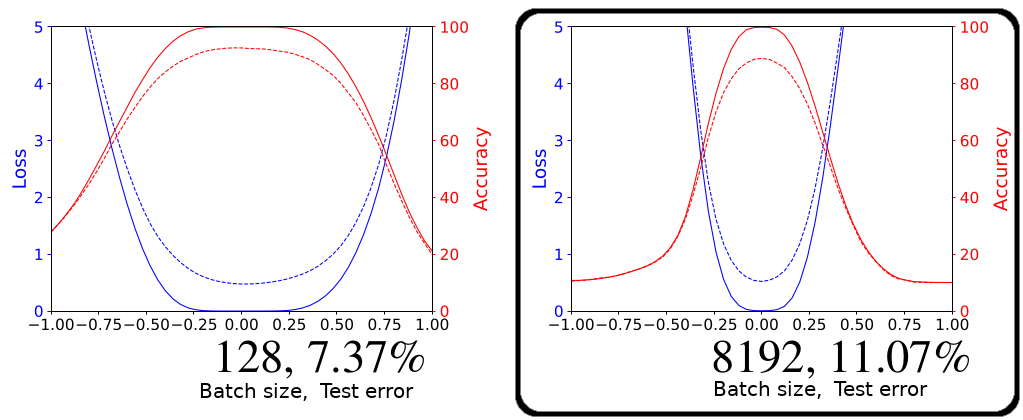
\includegraphics[width=.85\linewidth]{figures/batch_size_normalized_2.png}
	%\caption{Loss landscape around $\hat{\theta }$ for two models trained on different batch sizes.}
\end{figure}
\begin{itemize}
	\item Loss landscape around $\hat{\theta }$
	\item For batch size $128$ versus $8192$
	\item Smaller batch size indeed has flatter minimum
	\item and lower test error
	\item Slight difference in 'flatness'
\end{itemize}
\tiny\color{lightgray}Image source: Visualizing the loss landscape of neural nets - Li et al.
\end{frame}




%\begin{frame}
%\frametitle{Methods}
%\framesubtitle{2D with Filter Normalization - Observations}
%\begin{itemize}
%	\item Loss landscape can be quite convex
%	\item Architecture matters
%	\item Flatter minima generalize slightly better
%	\begin{itemize}
%		\item This is backed by analysis of Hessian at different $\hat{\theta}$
%	\end{itemize}
%\end{itemize}
%\end{frame} 


\begin{frame}
\frametitle{Methods}
\framesubtitle{2D with Filter Normalization - Challenges}
\begin{itemize}
	\item High computational cost
	\item No experiments on recurrent architectures (so far)
	\item Only models that perform well on benchmark datasets were investigated
	\item Not perfectly clear whether findings hold for other models %on non benchmark tasks
\end{itemize}
\end{frame} 


\begin{frame}
\frametitle{What did we learn from visualizations?}
\framesubtitle{Summary}
\begin{itemize}%\setlength\itemsep{1.5em}
	\item Roughly convex loss landscape
	\item Depending on architecture
	\item Relation between flatness and generalization
	\begin{itemize}
		\item Backed by further analysis of Hessians at minima
	\end{itemize}
%	\item Optima with good generalization lie in flat minima
	\item How can we put these findings to use?
	\begin{itemize}%\setlength\itemsep{1.5em}
		\item Exploit convex structure
		\item Build optimizer that prefers flat minima
	\end{itemize}
\end{itemize}
\end{frame} 


%\begin{frame}
%\frametitle{Examples}
%\framesubtitle{What are we looking for?}
%\begin{itemize}%\setlength\itemsep{1.5em}
%	\item Exploit convex structure
%	\item Optimzer that prefers flat minima
%\end{itemize}
%\end{frame} 



\begin{frame}
\frametitle{Examples}
\framesubtitle{PAL - Parabolic Approximation Line Search - Mutschler \& Zell}
\begin{itemize}%\setlength\itemsep{1.5em}
%	\item Assuming convex 
%	 (in update direction)
	\item Show loss in gradient direction is mostly convex
	\item Well suited for parabolic approximation
	\item Adjust step size according to shape of loss
\end{itemize}
\end{frame} 

\begin{frame}
\frametitle{Examples}
\framesubtitle{PAL - Intuition}
\begin{figure}
	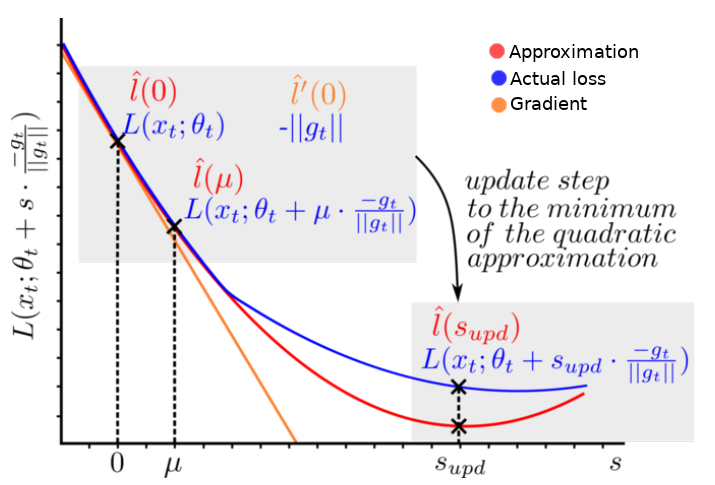
\includegraphics[width=.5\linewidth]{figures/pal_1.png}
\end{figure} 	
\begin{itemize}%\setlength\itemsep{1.5em}
	\item Take measurements
	\begin{itemize}
		\item current loss $l_t(0)$
		\item derivative in gradient direction $l_t'(0)$
		\item loss at measuring distance $l_t(\mu)$
	\end{itemize}
	
%	\item Approximate parabola
%	\item Make step according to approximated parabola
\end{itemize}
\tiny\color{lightgray}Image source: Parabolic Approximation Line Search for DNNs - Mutschler \& Zell
\end{frame}

\begin{frame}
\frametitle{Examples}
\framesubtitle{PAL - Update rule}
\begin{align*}
	\hat{l_t}(s) &= \color{blue}a\color{black}s^2 \color{black}+ \color{red}b\color{black}s \color{black} + c\\
	\text{with parameters } \color{blue}a &=\color{blue}\underbrace{\frac{l_t(\mu) - l_t(0) - l'(0)\mu}{\mu^2}}_{curvature}\\
	\color{red} b&= \color{red}\underbrace{l_t'(0)}_{shift}\\
	c &= \underbrace{l_t(0)}_{height}
\end{align*}
\begin{itemize}
	\item $\rightarrow$ Jump to minimum of approximated parabola
\end{itemize}
%Using the approximation, the update is
%\begin{align*}
%	s_{upd_t} = - \frac{\hat{l_t}'(0)}{\hat{l_t}''(0)} = -\frac{b}{2a} = \frac{-l'_t(0)}{ 2\frac{l_t(\mu) - l_t(0) - l'(0)\mu}{\mu^2}}
%\end{align*}
\end{frame}

\begin{frame}
\frametitle{Examples}
\framesubtitle{PAL - Results}
\begin{figure}
	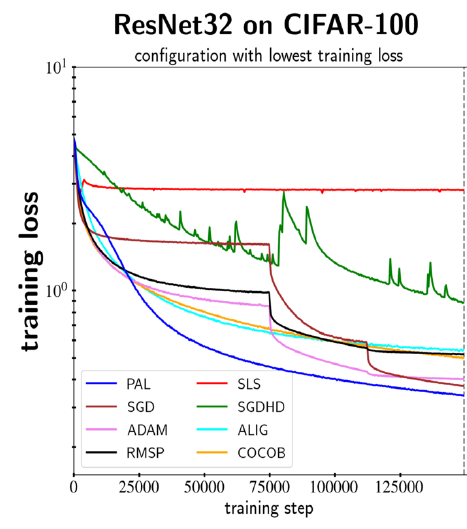
\includegraphics[width=.6\linewidth]{figures/pal_2.png}
\end{figure}
%\begin{itemize}%\setlength\itemsep{1.5em}
%	\item 
%\end{itemize}
\tiny\color{lightgray}Image source: Parabolic Approximation Line Search for DNNs - Mutschler \& Zell
\end{frame}

\begin{frame}
\frametitle{Examples}
\framesubtitle{Entropy-SGD - Bias towards wide valleys - Chaudari et al.}
\begin{itemize}%\setlength\itemsep{1.5em}
	\item How to tell apart good minima from bad minima?
	\begin{itemize}
		\item -> flatness
	\end{itemize}
	\item Propose new metric - Local entropy
	\item Measures 'flatness' of valley
	\item Maximize this

	%\item Inspiration from physics
	%\item continuous time scale 
	%\item Fokker-Planck Equation
	%\item Steepest descent on Wasserstein metric
\end{itemize}
\end{frame} 




%\begin{frame}
%\frametitle{Examples}
%\framesubtitle{Entropy-SGD - Results}
%\begin{figure}
%	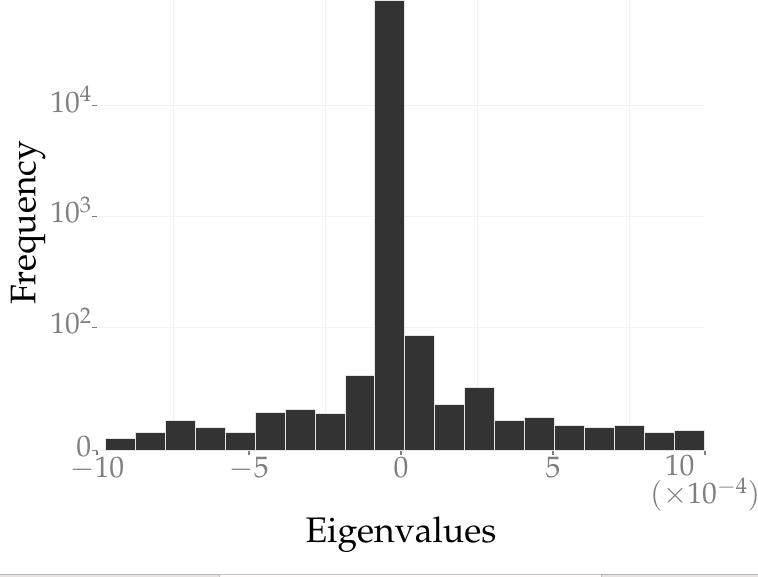
\includegraphics[width=.6\linewidth]{figures/eigenspectrum.png}
%\end{figure}
%\begin{itemize}%\setlength\itemsep{1.5em}
%	\item 
%\end{itemize}
%\tiny\color{lightgray}Image source: Entropy-SGD Biasing Gradient Descent Into Wide Valleys - Chaudari et al.
%\end{frame}
\begin{frame}
\frametitle{Examples}
\framesubtitle{Entropy-SGD - Results}
\begin{figure}
	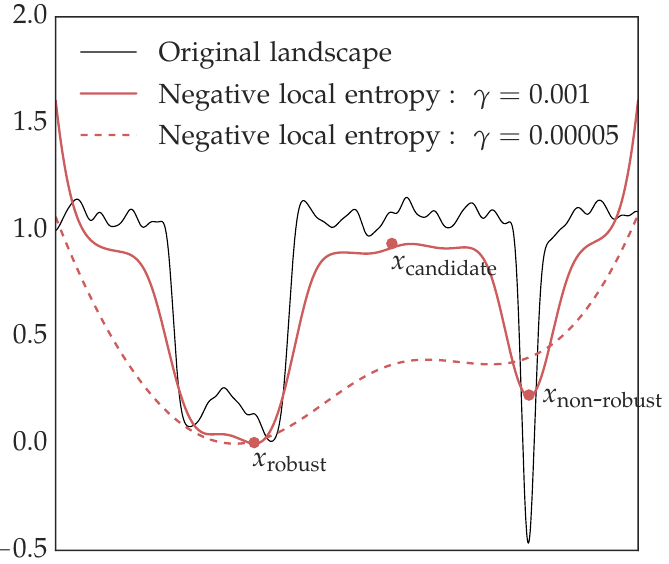
\includegraphics[width=.7\linewidth]{figures/entropy_1.png}
\end{figure}
%\begin{itemize}%\setlength\itemsep{1.5em}
%	\item 
%\end{itemize}
\tiny\color{lightgray}Image source: Entropy-SGD Biasing Gradient Descent Into Wide Valleys - Chaudari et al.
\end{frame}



\begin{frame}
\frametitle{Examples}
\framesubtitle{Entropy-SGD - Results}
\begin{itemize}
	\item Nested optimization loop
	\item At every step, estimate volume of good parameter cofigurations in neighborhood
%	\item At every SGD step, scan volume of different parameter configurations in neighborhood
	\item the larger the volume, the flatter the minimum
	\item Scope hyperparameter $\gamma$
	\begin{itemize}
			\item Determines 'how far to look for configurations'
		\item for $\gamma \rightarrow \infty$, approaches regular loss landscape
		\item for $\gamma \rightarrow 0$, approaches uniform distribution
	\end{itemize}
\end{itemize}
%\begin{align*}
%	\mathcal{L}_{Local\;Entropy}(W, \gamma) = \frac{1}{\beta}log \int exp( -\beta \mathcal{L}(x') - \frac{\gamma}{2} ||W - W'||^2_2)dx'
%\end{align*}
\end{frame}




\begin{frame}
\frametitle{Examples}
\framesubtitle{Entropy-SGD - Results}
\begin{figure}
	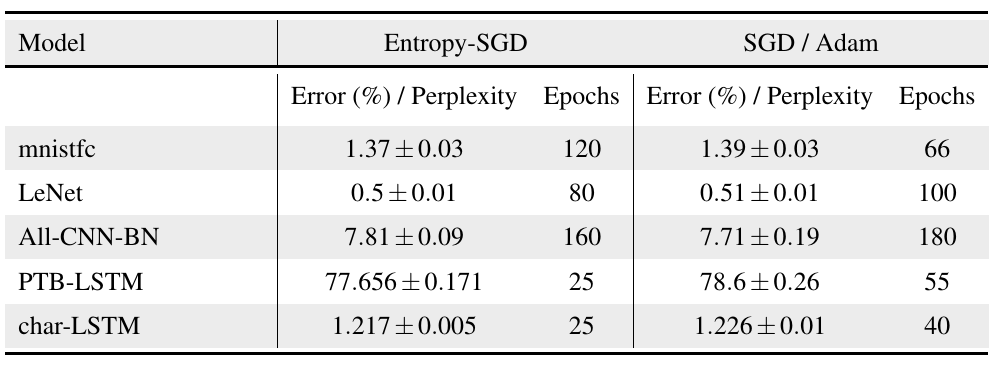
\includegraphics[width=.9\linewidth]{figures/entropy_results.png}
\end{figure}
\begin{itemize}%\setlength\itemsep{1.5em}
	\item Entropy-SGD has lower error/perplexity in most settings 
\end{itemize}
\tiny\color{lightgray}Table source: Entropy-SGD Biasing Gradient Descent Into Wide Valleys - Chaudari et al.
\end{frame}


\begin{frame}
\frametitle{Takeaways}
\framesubtitle{What did we learn?}
\begin{itemize}%\setlength\itemsep{1.5em}
%	\item SGD is great
	\item Visualizing helps with intuition% and can help open new directions
	\item provides good foundation for empirical analysis
	\item helps building better optimizers
	\item \color{red}Questions for you:
	\begin{itemize}
		%\item Is LLV a promising field
		\item \color{red}Is LLV worth the effort or is it just pretty pictures?
%		\item Can it be used for more empirical approaches?
		\item \color{red}How does it compare to grid search?
		\item \color{red}What would you want in a good loss landscape visualization?
	\end{itemize}
\end{itemize}
\end{frame} 




\begin{frame}
\frametitle{References}
%\framesubtitle{}
\begin{itemize}%\setlength\itemsep{1.5em}
	\item Xing, C., Arpit, D., Tsirigotis, C. and Bengio, Y., 2018. A walk with sgd. arXiv preprint arXiv:1802.08770.
	\item Chaudhari, P., Choromanska, A., Soatto, S., LeCun, Y., Baldassi, C., Borgs, C., Chayes, J., Sagun, L. and Zecchina, R., 2019. Entropy-sgd: Biasing gradient descent into wide valleys. Journal of Statistical Mechanics: Theory and Experiment, 2019(12), p.124018.
	\item Mutschler, M. and Zell, A., 2019. Parabolic Approximation Line Search: An efficient and effective line search approach for DNNs. arXiv preprint arXiv:1903.11991.
	\item Li, H., Xu, Z., Taylor, G., Studer, C. and Goldstein, T., 2018. Visualizing the loss landscape of neural nets. In Advances in neural information processing systems (pp. 6389-6399).
\end{itemize}
\end{frame} 
\begin{frame}
\frametitle{References}
%\framesubtitle{}
\begin{itemize}%\setlength\itemsep{1.5em}
	\item Goodfellow, I.J., Vinyals, O. and Saxe, A.M., 2014. Qualitatively characterizing neural network optimization problems. arXiv preprint arXiv:1412.6544.
	\item Baldassi, C., Borgs, C., Chayes, J.T., Ingrosso, A., Lucibello, C., Saglietti, L. and Zecchina, R., 2016. Unreasonable effectiveness of learning neural networks: From accessible states and robust ensembles to basic algorithmic schemes. Proceedings of the National Academy of Sciences, 113(48), pp.E7655-E7662.
	\item Hochreiter, S. and Schmidhuber, J., 1997. Flat minima. Neural Computation, 9(1), pp.1-42.
\end{itemize}
\end{frame} 



\end{document}
